\documentclass{article}
\usepackage[utf8]{inputenc}

\title{Monitoring and Recovering System for the Optimisation Process in Engineering}
    
\author{Mathieu Dutour, Miguel Martínez, Jakub Baron, Léo Raimondjean}
\date{March 2015}

\usepackage{natbib}
\usepackage{graphicx}

\begin{document}

\maketitle

\tableofcontents

\section{Introduction}
The purpose of this project is to develop a distributed system for monitoring a workflow process. We will be working to optimize a complex computational problem which will require the work of several solver systems whose objective will be the optimization of the design of an aerofoil in terms of a given set of parameters that will ultimately affect the lift and drag of an aircraft. The aim will be to enhance these parameters in such a way that the drag of the aircraft is minimized while the lift is maximized. The system will be web-based facilitating its use and access by anyone through any internet-enabled device.


\section{Airflow Optimization Problem}

For this project we will compute the lift and drag forces for a symmetrical 4-digit NACA airfoil. Considering the lift coefficient to be

\begin{equation}
L = \frac{1}{2}\rho v^2 A C_L
\end{equation}

using the thin airfoil theory method, given that the lift coefficient is known for a certain angle of attack.

where

\begin{itemize}
  \item L is lift force,
  \item $\rho$ is air density,
  \item v is true airspeed,
  \item A is platform area, and
  \item $C_L$ is the lift coefficient at the desired angle of attack
\end{itemize}


\begin{figure}[h!]
\centering
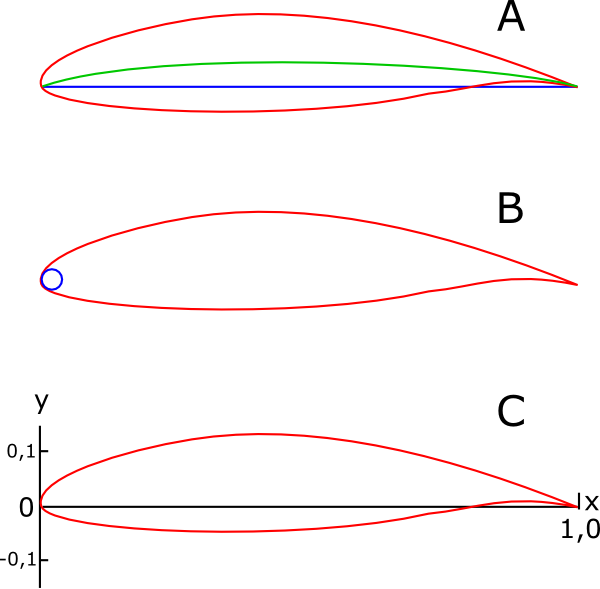
\includegraphics[scale=0.15]{airfoil.png}
\caption{NACA airfoil \cite{airfoil_wikipedia}}
\label{fig:nacaairfoil}
\end{figure}


\textit{ADD MORE AWESOME SCIENTIFIC PHYSICS STUFF HERE!!}


\section{Requirements}

The following sections pertain to the analysis of the functional and non-functional requirements of this specific software system.

\subsection{Functional Requirements}


\par
\textbf{Intuitive User Interface:}
One of the requirements of this system is that a intuitive user interface be built to be able to manage and control the underlying system and easily access log entries, optimization data and more. The user interface was built to be highly configurable and customizable allowing the user to easily navigate the interface through a series of self-explanatory icons for navigation which are always present on the left-hand side of the screen.\\\par

\noindent\textbf{Start optimization execution:}
The web application in charge of managing the execution of the optimization procedures naturally allows for an authenticated user or administrator to start a brand new execution process. The administrator can also view previously recorded executions along with all their associated data.\\\par

\noindent\textbf{Provide a log of important actions within the system:}
The user interface also provides a way of accessing all logged data from the system such as when a new account is created, when a connection from a user is registered, when optimization procedures are created, executed, deleted, etc.



\subsection{Non-Functional Requirements}

\par
\textbf{System Resources:}
\\\par

\noindent\textbf{Product Requirements:}
\\\par

\noindent\textbf{External Requirements:}
\\\par


\subsection{Software System Characteristics}


\begin{itemize}
   \item  Reliability: A description of  how our system is reliable goes here...

   \item  \textit{Security:} We use SSH for authentication by connecting to the Astral cluster to make sure that the system is only used by a Cranfield team, but is developed in a way that makes it really easy to modify it for other authentication methods. SSH is a cryptographic network protocol that ensure that any data that goes through the wire in the authentication process is encrypted, by means of establishing a secure channel over the network which by definition is open to probing and attacks.

   \item  \textit{Usability:} A description of  how our system is usable goes here...

   \item  \textit{Performance:} A description of  how our system performs well goes here...

   \item  \textit{Portability:} The system, due to having been built on top of a web stack makes it extremely portable. Any device with a connection to the Internet can access the interface and launch new optimizations right away, check logs for any required information and perform any relevant changes.

\end{itemize}



\section{Technology}

\subsection{Meteor}

Meteor is a realtime web application framework which supports realtime interaction and reactivity out-of-the-box.

\subsubsection{Underlying Principles}

Meteor has some rather interesting characteristics that separate it from other platforms. It optimizes the quantity of data that needs to be sent to the client over the network. Since the client and the server execute the same exact code, Meteor doesn't send HTML through the wire, instead it sends the necessary data needed to render the page. It allows for the web application to be built using Javascript as the common programming language making it extremely lightweight and practically able to be executed in any browser that has Javascript enabled, which most do by default.\\\par

\noindent Another interesting characteristic of Meteor is that the database, where we store user information, optimization and log data, is accessible from both client and server. Moreover they are automatically synchronized, which means that any change that occurs in the database is automatically rendered in the client's view. On these terms, Meteor introduces a concept called ``latency compensation``, which as its name indicates is a method to alleviate network latency. It consists in the emulation of a subset of the Mongo database from the server in the client itself. This way a copy of the necessary subset of data resides in the client and any changes are automatically propagated to the other Mongo instances. This prefetching of data makes it look like a call to the server is getting a response instantly.



\section{Conclusion}

\bibliographystyle{unsrt}
\bibliography{references}

\end{document}
